\documentclass{beamer}

\usepackage[english]{babel}
\usepackage{xcolor}
\usepackage{amsmath}
\usepackage{amssymb}
\usepackage{comment}

\usepackage{tikz}
\usepackage{pgfplots}
\usepackage{pgfplotstable}
\usetikzlibrary{plotmarks,arrows,shapes,backgrounds}

%\usefonttheme{serif}
%\usepackage{palatino}
\usetheme{Rochester}
\usecolortheme{beaver}
\beamertemplatenavigationsymbolsempty

\title{ 
    ~\\~\\ 
    {\huge AdaProp} 
    \\~\\
    {\large Adaptive Propositionalisation of Multi-Instance Data Towards Image Classification}
    \\~
}
\author{~\\~\\Siva~Manoharan\\~\\Supervisor:~Dr~Eibe~Frank}
\date{} %% no date

%% Customizing colours:
\colorlet{primaryRed}{darkred!60!black}       %% For most Reds
\colorlet{secondaryRed}{darkred!80!black}     %% When Red is surrounded by grey
\colorlet{bgWhite}{white!97!black}            %% Near white, for page backgrounds
\colorlet{headerGrey}{white!90!black}         %% For Header backgrounds
\colorlet{fillGrey}{white!80!black}           %% For filling areas, e.g. chart areas
\colorlet{edgeGrey}{white!60!black}           %% For increasing apparent sharpness

\setbeamercolor*{item}{fg=primaryRed}         %% Bullet points
\setbeamercolor{title}{fg=secondaryRed}       
\setbeamercolor{background canvas}{bg=bgWhite}
\setbeamercolor{headline}{bg=headerGrey}
\setbeamertemplate{headline}[text line]{%
  \begin{beamercolorbox}%
      [wd=\paperwidth,ht=2cm]{headline}%
  \end{beamercolorbox}%
}

%% A Macro for a image and a caption
%% args: image, caption
\newcommand{\CenteredImage}[1]{%
    \begin{center} 
        \includegraphics[scale=0.25]{img/#1}
    \end{center}
}

%% A Macro for a image and a caption in a column
%% args: image, caption
\newcommand{\ImageAndCaptionColumn}[2]{%
    \begin{column}{.5\textwidth}
        \begin{center} 
            \includegraphics[scale=0.25]{img/#1} \\~\\ 
            {\Large #2}
        \end{center} 
    \end{column}
}

%% A Macro for frame template: a bullet point above two images, each with caption
%% args: bullet-text, img-left, caption-left, img-right, caption-right
\newcommand{\TextAndTwoImageFrame}[5]{%
    %% Default spacing is too large for just one bullet point.
    %% Reduce it:
    \vspace{-0.5cm}    
    
    \begin{itemize}
        \item #1
    \end{itemize}
    
    \vspace{-0.5cm} %% again, reducing spacing
    
    %% Two columns of image+caption pairs:
    \begin{columns}[T]
        \ImageAndCaptionColumn{#2}{#3}
        \ImageAndCaptionColumn{#4}{#5}
    \end{columns}
}

%% A Macro for frame template: 3 bullet points
%% args: bullet1, bullet2, bullet3
\newcommand{\ThreeBulletFrame}[3]{%
    \begin{itemize}
        \item {#1} \\ ~
        \item {#2} \\ ~
        \item {#3}
    \end{itemize}
}

%% A Macro for a column and line graph for our datasets:
%% args: bg-label, bg-coords, fg-label, fg-coords ; where
%%    bg: background datapoints, fg: foreground datapoints.
\newcommand{\ColumnAndLineGraph}[4]{%
    \begin{axis}[
        %% Fixed size graph
        width=11cm, height=7cm, bar width=0.35cm,
%
        %% draw only left and bottom lines
        axis x line*=bottom, axis y line*=left, draw=edgeGrey,
%
        %% y-axis: 40-95, with major=10, minor=5
        ymin=40, ymax=95, minor y tick num=1,  ytick={50,60,70,80,90},
        axis y discontinuity=crunch, ylabel={Accuracy (\%)},
%
        %% x-axis: category axis
        symbolic x coords={atoms,bonds,chains,musk1,musk2,trx,tiger,fox,eleph,people,bikes,cars},
        xtick=data, x tick label style={rotate=90,anchor=east}, 
%
        %% Legend: at bottom right, place line first, then bar.
        reverse legend, legend pos=south east
    ]
 
        %% Background bar plot
        \addplot[ybar,fill=fillGrey, draw=edgeGrey, area legend] 
            coordinates {#2};
        \addlegendentry{#1}
        
        %% Foreground line plot
        \addplot+[ycomb,mark=-,draw=primaryRed,very thick,mark size=0.175cm, line legend] 
            coordinates {#4};
        \addlegendentry{#3}
    \end{axis}
}

%% A Macro for drawing a Bag Of Vectors inside a TikZpicture.
%% Args: 
%%    xEllipse, yEllipse, yTopDots, yFirstVec, 
%%    yMidDots, ySecondVec, yBottomDots, yLabel
\newcommand{\BagOfVectors}[8]{%
    \draw [dashed, fill=white!92!black, draw=edgeGrey, very thick] (#1,#2) ellipse (0.8cm and 1.9cm);
    \node at (#1,#3) { \Large $\vdots$ };
    \node at (#1,#4) {\large $\left\langle {X_i} \right\rangle$};
    \node at (#1,#5) { \Large $\vdots$ };
    \node at (#1,#6) {\large $\left\langle {X_j} \right\rangle$};
    \node at (#1,#7) { \Large $\vdots$ };        
    \node at (#1,#8) { \Large Bag of vectors };
}

%% A Macro for horizontal, red, thick arrows.
%% Args: x-start, x-end, y-coord
\newcommand{\HorizArrow}[3]{%
    \path [->, primaryRed, ultra thick] (#1,#3) edge (#2,#3);
}

%% uncomment for logo
%\pgfdeclareimage[height=0.5cm]{university-logo}{university-logo-filename}
%\logo{\pgfuseimage{university-logo}}

\begin{document}

%% remove header bar for the titlepage
{
    \makeatletter
        \setbeamercolor{headline}{bg=bgWhite}
        \def\beamer@entrycode{\vspace*{-0.8\headheight}}
    \makeatother

    \begin{frame}
        \titlepage
    \end{frame}
}

\begin{frame}{Image Classification}

    \TextAndTwoImageFrame{
        Does the Image contain a specific object?
    }{cars1}{Car}{none1}{No car}
    
\end{frame}

\begin{frame}{Image Classification}

    \TextAndTwoImageFrame{
        Not easy in practice (for computers)
    }{cars3}{Not in Foreground}{cars2}{Partial Occlusion}
    
\end{frame}

\begin{frame}{Multi-Instance Learning}
    
    \vspace{-0.355cm}
    \begin{itemize}
        \item Natural fit for Image Classification %% (also Chemical, Text)
    \end{itemize}
    \vspace{0.215cm}
    
    \makebox[\linewidth]{\parbox{11.5cm}{%
        \begin{tikzpicture}%[every text node part/.style={align=center}]
        
        %% include the car picture
        \node [inner sep=0pt,below right] {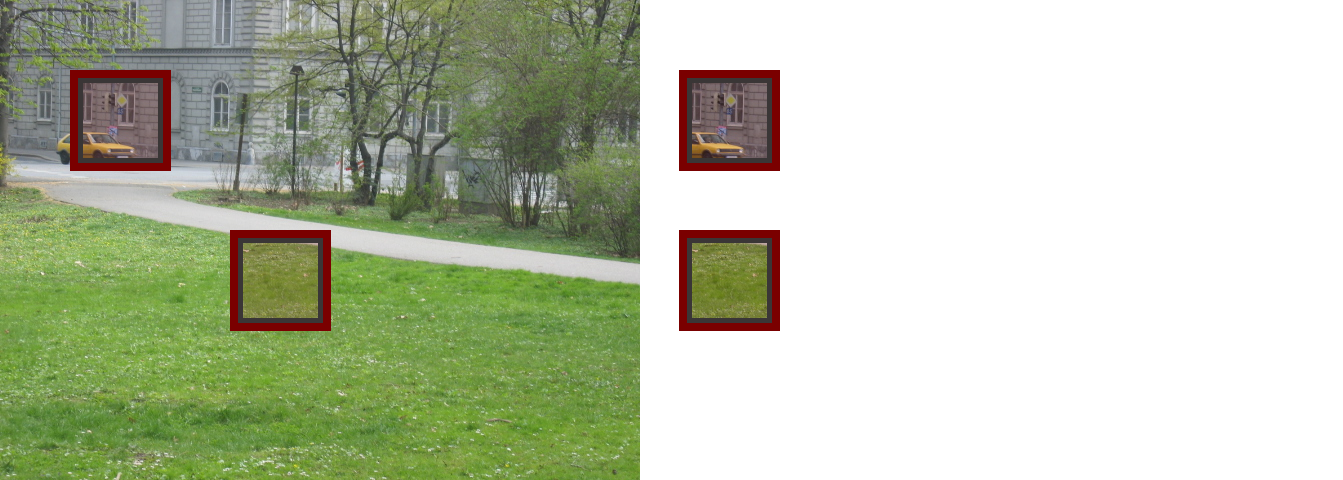
\includegraphics[scale=0.25]{img/cars4}};
        
        %% Intermediate points
        \def\xZ{5.77};
        \def\xY{6.65};
        \def\xX{10.00};        
        
        %% Define some points: 'A' near the car, 'B' away from the car
        \def\yA{-1.05};
        \def\yB{-2.40};
        
        %% Arrows from image to floats
        \HorizArrow{1.45}{\xZ}{\yA};
        \HorizArrow{2.80}{\xZ}{\yB};
      
        %% Captions:
        \def\yCaption{-5};
        \node at (3.00, \yCaption) { \Large Sub-regions };

        %% Draw the bag of vectors:
        \uncover<2>{
            \BagOfVectors{10.4}{-1.8}{-0.30}{-1.10}{-1.60}{-2.45}{-3.00}{\yCaption}
            \HorizArrow{\xY}{\xX}{\yA}; 
            \HorizArrow{\xY}{\xX}{\yB};     
            \node[%draw=edgeGrey, dashed, very thick,text height=1cm, text depth=1cm,
                text width=2.2cm, 
                every text node part/.style={align=center}] at (8.2, -1.7) 
                { \Large Feature Extraction };
        }
        \end{tikzpicture}
    }}

\end{frame}

\begin{frame}{Propositionalisation}

    \makebox[\linewidth]{\parbox{11.5cm}{%
        \tikzstyle{background grid}=[draw, black!50,step=0.5cm]
        \begin{tikzpicture}%[show background grid]%[every text node part/.style={align=center}]
        
        %% Bag of vectors ellipse:
        \def\xEllipse{1.5}
        \def\yBase{-1.8};     
        \def\yCaption{-5};
        \BagOfVectors{\xEllipse}{\yBase}{-0.30}{-1.10}{-1.60}{-2.45}{-3.00}{\yCaption}
        
        %% Propositionalisation node:
        \def\xProp{4.5};
        \node[draw=edgeGrey, very thick, text height=1cm, text depth=0.7cm,
            rotate=90, text width=4.5cm,
            every text node part/.style={align=center}]
            at (\xProp, \yBase)
            {\Large Propositionalisation};
            
        %% Single vector circle:
        \def\xCirc{7.25};        
        \draw [dashed, fill=white!92!black, draw=edgeGrey, very thick] (\xCirc,\yBase) circle (0.7cm);
        \node at (\xCirc,\yBase) { \large $\left\langle {Y} \right\rangle$ };
        \node at (\xCirc,\yCaption) { \Large Single vector };
        
        %% Arrows:
        \def\yA{-1.095};
        \def\yB{-2.445};
        \def\xZ{1.90};
        \def\xY{3.45};
        \HorizArrow{\xZ}{\xY}{\yA};
        \HorizArrow{\xZ}{\xY}{\yB};
        \HorizArrow{5.50}{6.475}{\yBase};
        
        %% Base Learner node:
        \uncover<2->{
            \HorizArrow{7.95}{8.95}{\yBase};
            \node[draw=edgeGrey, very thick, text height=0.85cm, text depth=0.85cm,
                rotate=90, text width=4.5cm,
                every text node part/.style={align=center}]
                at (10, \yBase)
                {\Large Standard ML Algorithm};          
        }
        
        %% Adaptive arrow
        \def\yAda{0};
        \only<3>{
            \frametitle{Adaptive Propositionalisation}       
        }
        \uncover<3>{
            \path [->, primaryRed, ultra thick, line width=0.1cm] (9,0) edge (5.55,0);
            \node[color=primaryRed] at (\xCirc,0.3) { \Large Adaptive };
        }
        
    \end{tikzpicture}
    }}
            
\end{frame}

\begin{comment}
\begin{frame}{Multi-Instance Learning}
    \ThreeBulletFrame
        {Natural for Image Classification}
        {Text Classification and Chemical datasets}
        {Key: Bags of Instances}
\end{frame}

\begin{frame}{Propositionalisation}
    \ThreeBulletFrame
        {Multi-instance $\to$ Single-instance}
        {Advantage: Existing algorithms}
        {Disadvantage: Lossy conversion}   
\end{frame}

\begin{frame}{AdaProp: Adaptive Propositionalisation}
    \ThreeBulletFrame
        {Use the base learner}
        {Tree of decisions / partitions}
        {Count by region}
\end{frame}
\end{comment}


\begin{frame}{WEKA}

  \vspace{-0.5cm}
  \CenteredImage{weka3}
  
\end{frame}

\begin{comment}
\begin{frame}{Impact of Parameter Selection}

    \begin{tikzpicture}
        \ColumnAndLineGraph{Without}{
            (atoms,77.14)  (bonds,84.40)  (chains,85.81)
            (musk1,73.39)  (musk2,73.30)  (trx,85.36)
            (tiger,75.70)  (fox,65.95)    (eleph,73.30)
            (people,75.6)  (bikes,75.35)  (cars,68.54)
        }{With ParamSel}{
            (atoms,84.49)  (bonds,87.48)  (chains,86.60)
            (musk1,76.28)  (musk2,74.48)  (trx,86.61)
            (tiger,79.60)  (fox,65.95)    (eleph,75.90)
            (people,76.27) (bikes,77.24)  (cars,68.76)
        }
    \end{tikzpicture} 

\end{frame}
\end{comment}

\begin{frame}{AdaProp vs. Other MI algorithms}

    \begin{tikzpicture}
        \ColumnAndLineGraph{Others}{
            (atoms,83.90)  (bonds,87.96)  (chains,88.56)
            (musk1,90.68)  (musk2,85.89)  (trx,90.32)
            (tiger,84.30)  (fox,67.00)    (eleph,85.50)
            (people,82.60) (bikes,83.50)  (cars,77.22)
        }{AdaProp}{
            (atoms,87.52)  (bonds,89.44)  (chains,89.86)
            (musk1,85.76)  (musk2,82.26)  (trx,88.64)
            (tiger,84.20)  (fox,68.20)    (eleph,84.75)
            (people,81.88) (bikes,82.50)  (cars,77.08)
        }
    \end{tikzpicture}
    
\end{frame}

\begin{frame}{Summary}

  % must be *very short*.
  \begin{itemize}
  \item
      MI representation is \alert{natural} for Image Classification. \\ ~
  \item
      AdaProp propositionalises MI data using the \alert{base learner}. \\ ~
  \item
      \alert{Comparable performance} to other MI algorithms. % TODO need this?
  \end{itemize}
  
\end{frame}

\end{document}


